\section{次梯度方法}
\label{sec:opt-ns-subgradient-methods}

上一节说明了尖点处保留的是一整组支撑斜率。实际的计算程序通常拿不到整组斜率：给定查询点，它返回函数值和其中一条次梯度。本节研究只凭这样的信息怎样推进。最直接的做法是把梯度下降中的梯度换成次梯度；我们会看到，这一替换保留了“靠近最小点”的性质，却失去了“目标逐轮下降”的性质，所以必须重新规定算法返回哪一个点、报告什么误差。

\subsection{更新与返回对象}
\label{sec:opt-ns-subgradient-update}

设$f:\mathbb R^d\to\mathbb R$是凸函数（在全空间取有限值，因而每一点都有次梯度），计算程序对任意查询点$\bm x$返回$f(\bm x)$和某个$\bm g\in\partial f(\bm x)$。我们不能假定返回的是哪一条次梯度；分析必须对任意选择成立。\term{次梯度法}（subgradient method）的一轮更新是
\begin{equation}
 \bm x^{(t+1)}=\bm x^{(t)}-\eta^{(t)}\bm g^{(t)},\qquad\bm g^{(t)}\in\partial f(\bm x^{(t)}),
 \label{eq:opt-ns-subgradient-update}
\end{equation}
其中$\eta^{(t)}>0$是预先规定的步长。目标若取扩展实值，更新后的点可能落到$\operatorname{dom}f$之外，那里既没有有限函数值也没有次梯度；这时需要把更新点投影回可行集，相应的投影次梯度法在第~\ref{chap:constrained-optimization}章讨论。本节只处理全空间有限值的目标。

\paragraph{负次梯度未必是下降方向}
梯度下降之所以能用小步长保证下降，是因为$-\nabla f(\bm x)$与目标的局部变化相匹配：沿它走一小步$s$，一阶变化是$-s\lVert\nabla f(\bm x)\rVert_2^2<0$。次梯度不再有这种匹配。先看一维的例子：$f(x)=|x|$，从$x^{(0)}=0.2$以步长$1$沿$-\operatorname{sign}(x)$走，得到$x^{(1)}=-0.8$，目标从$0.2$升到$0.8$。这里的失败可以归咎于步长太大、跨过了尖点。

更本质的情况是，有些负次梯度方向对任何正步长都会使目标上升。取$f(\bm x)=|x_1|+2|x_2|$与$\bm x=(1,0)^\top$。由可分规则~\eqref{eq:opt-ns-separable-subdifferential}，$\partial f(\bm x)=\{1\}\times[-2,2]$，所以$\bm g=(1,2)^\top$是一条合法的次梯度。沿$-\bm g$走步长$s\in(0,1)$，
\[
 f(\bm x-s\bm g)=|1-s|+2|-2s|=1+3s>1=f(\bm x),
\]
无论$s$多小，目标都上升。同一点的另一条次梯度$(1,0)^\top$却是下降方向。图~\ref{fig:opt-ns-subgrad-not-descent}把这一现象画在等高线上：红色箭头$-\bm g$离开了$f=1$的菱形等高线，进入了目标更大的区域。

\begin{figure}[!htbp]
  \centering
  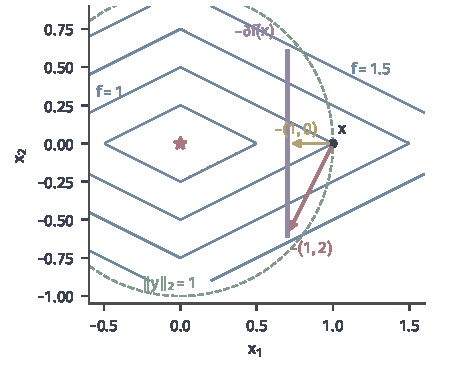
\includegraphics[width=80mm]{figures/03-optimization-evolution-and-signals/01-optimization/matplotlib/c4-subgrad-not-descent/figure.pdf}
  \caption{负次梯度方向可能使目标上升，却仍然靠近最小点。蓝色菱形是$f(\bm x)=|x_1|+2|x_2|$的等高线（$f=0.5,1,1.5,2$），红星是最小点$\bm 0$。在$\bm x=(1,0)^\top$处，次微分$\{1\}\times[-2,2]$的负向（按$0.3$倍缩放）画成紫色竖线段。红色箭头沿$-(1,2)^\top$，越出$f=1$的等高线，目标上升；黄色箭头沿$-(1,0)^\top$，目标下降。绿色虚线是以最小点为圆心、过$\bm x$的圆：两支箭头的终点都在圆内。}
  \label{fig:opt-ns-subgrad-not-descent}
\end{figure}

\paragraph{负次梯度靠近最小点}
图中还有一个容易忽略的事实：红色箭头虽然使目标上升，却进入了以最小点为圆心、过当前点的圆内。这不是巧合。设$\bm x^\star$是任一最小点，$\bm g\in\partial f(\bm x)$，把支撑不等式~\eqref{eq:opt-ns-subgradient-inequality}用于$\bm y=\bm x^\star$，得$\langle\bm g,\bm x-\bm x^\star\rangle\geq f(\bm x)-f^\star$。于是
\begin{equation}
 \begin{aligned}
 \lVert\bm x-s\bm g-\bm x^\star\rVert_2^2
 &=\lVert\bm x-\bm x^\star\rVert_2^2-2s\langle\bm g,\bm x-\bm x^\star\rangle+s^2\lVert\bm g\rVert_2^2\\
 &\leq\lVert\bm x-\bm x^\star\rVert_2^2-2s\bigl(f(\bm x)-f^\star\bigr)+s^2\lVert\bm g\rVert_2^2.
 \end{aligned}
 \label{eq:opt-ns-distance-one-step}
\end{equation}
其中$s>0$是步长。只要$\bm x$不是最小点、$s$足够小，右端就严格小于$\lVert\bm x-\bm x^\star\rVert_2^2$。在上面的例子中，$\lVert\bm x-s\bm g\rVert_2^2=(1-s)^2+4s^2=1-2s+5s^2$，$0<s<2/5$时小于$1$。次梯度方法的进展是用到最小点的距离来衡量的，而不是用目标值；这一点决定了下面的返回规则和下一小节的分析。

\paragraph{历史最佳点与加权平均点}
既然目标值可以在某一轮上升，最后一个迭代点就不一定是目前找到的最好点。算法因此要维护一个返回对象，常用的有两种：历史最佳点$\bm x_{\mathrm{best}}^{(T)}$，即$\bm x^{(0)},\dots,\bm x^{(T-1)}$中目标值最小的一个；以及按步长加权的平均点
\[
 \bar{\bm x}^{(T)}=\frac{\sum_{t=0}^{T-1}\eta^{(t)}\bm x^{(t)}}{\sum_{t=0}^{T-1}\eta^{(t)}}.
\]
最佳点需要每轮的函数值；平均点不需要函数值，但要额外维护一个加权和。

\begin{algorithm}[次梯度法]
  \label{alg:opt-ns-subgradient}
  \begin{algorithmic}[1]
    \Require 在全空间有限的凸函数$f$的函数值与次梯度程序；初值$\bm x^{(0)}$；步长$\eta^{(0)},\dots,\eta^{(T-1)}>0$；预算$T$
    \Ensure 历史最佳点$\bm x_{\mathrm{best}}$、加权平均点$\bar{\bm x}$及相应目标值
    \State $f_{\mathrm{best}}\gets+\infty$，$\bm s\gets\bm 0$，$W\gets0$
    \For{$t=0,1,\dots,T-1$}
      \State 查询$f(\bm x^{(t)})$与一个$\bm g^{(t)}\in\partial f(\bm x^{(t)})$
      \If{$f(\bm x^{(t)})<f_{\mathrm{best}}$}
        \State $f_{\mathrm{best}}\gets f(\bm x^{(t)})$，$\bm x_{\mathrm{best}}\gets\bm x^{(t)}$
      \EndIf
      \If{$\bm g^{(t)}=\bm 0$}
        \State \Return $\bm x^{(t)}$（零次梯度已证明它是全局最小点）
      \EndIf
      \State $\bm s\gets\bm s+\eta^{(t)}\bm x^{(t)}$，$W\gets W+\eta^{(t)}$
      \State $\bm x^{(t+1)}\gets\bm x^{(t)}-\eta^{(t)}\bm g^{(t)}$
    \EndFor
    \State $\bar{\bm x}\gets\bm s/W$，计算$f(\bar{\bm x})$
    \State \Return $\bm x_{\mathrm{best}}$、$\bar{\bm x}$及其目标值
  \end{algorithmic}
\end{algorithm}

算法~\ref{alg:opt-ns-subgradient}每轮的代价是一次函数值与次梯度查询，加上$O(d)$的向量运算。注意更新顺序：当前点先参与最佳点和平均点的记录，然后才被替换；下一小节的误差界针对的正是这些被查询过的点。

\paragraph{停止时能报告什么}
光滑情形常用梯度范数作停止准则，次梯度范数却不能直接替代它。在$|x|$的原点，程序可能返回$g=1$，范数为$1$，而原点已是最优。真正与最优性对应的量是零到整个次微分的距离$\operatorname{dist}(\bm 0,\partial f(\bm x))=\min\{\lVert\bm g\rVert_2:\bm g\in\partial f(\bm x)\}$：由定理~\ref{thm:opt-ns-zero-subgradient}，它为零当且仅当$\bm x$最优。若它等于$\delta$，又已知$\lVert\bm x-\bm x^\star\rVert_2\leq R$，取达到最小范数的$\bm g$代入支撑不等式，得
\[
 f(\bm x)-f^\star\leq\langle\bm g,\bm x-\bm x^\star\rangle\leq\delta R.
\]
可惜计算这个距离需要整个次微分，而查询程序只给一条次梯度。

因此，次梯度法通常按预算停止，并报告返回点、其目标值和所依据的假设。若另有一个可信的下界$\ell\leq f^\star$（例如来自第~\ref{chap:constrained-optimization}章的对偶问题，或问题本身已知最小值非负），就可以报告可核验的目标间隙$f(\bm x_{\mathrm{best}})-\ell$，它是$f(\bm x_{\mathrm{best}})-f^\star$的上界。没有下界时，只能报告下一小节在相应假设下给出的理论界。

\subsection{步长与有限步误差}
\label{sec:opt-ns-subgradient-rate}

不等式~\eqref{eq:opt-ns-distance-one-step}说明每一步都在用目标差换取距离的减小，同时付出一项与步长平方成正比的代价。把这种交换沿迭代累加，就得到次梯度法的有限步误差界。

\begin{theorem}[次梯度法的有限步误差]
\label{thm:opt-ns-subgradient-rate}
设$f:\mathbb R^d\to\mathbb R$凸，最小点$\bm x^\star$存在，$\lVert\bm x^{(0)}-\bm x^\star\rVert_2\leq R$，并且算法实际取到的次梯度满足$\lVert\bm g^{(t)}\rVert_2\leq G$（$t=0,\dots,T-1$）。则
\begin{equation}
 \min_{0\leq t<T}f(\bm x^{(t)})-f^\star\leq\frac{R^2+G^2\sum_{t=0}^{T-1}(\eta^{(t)})^2}{2\sum_{t=0}^{T-1}\eta^{(t)}},
 \label{eq:opt-ns-subgradient-bound}
\end{equation}
并且加权平均点$\bar{\bm x}^{(T)}$满足同样的界。
\end{theorem}

\begin{proof}
对每一轮应用式~\eqref{eq:opt-ns-distance-one-step}（取$\bm x=\bm x^{(t)}$、$s=\eta^{(t)}$、$\bm g=\bm g^{(t)}$），整理得
\[
 2\eta^{(t)}\bigl(f(\bm x^{(t)})-f^\star\bigr)\leq\lVert\bm x^{(t)}-\bm x^\star\rVert_2^2-\lVert\bm x^{(t+1)}-\bm x^\star\rVert_2^2+(\eta^{(t)})^2G^2.
\]
对$t=0,\dots,T-1$求和，右端距离项逐项相消，只剩$\lVert\bm x^{(0)}-\bm x^\star\rVert_2^2-\lVert\bm x^{(T)}-\bm x^\star\rVert_2^2\leq R^2$，所以
\[
 2\sum_{t=0}^{T-1}\eta^{(t)}\bigl(f(\bm x^{(t)})-f^\star\bigr)\leq R^2+G^2\sum_{t=0}^{T-1}(\eta^{(t)})^2.
\]
左端每一项都不小于$2\eta^{(t)}\bigl(\min_sf(\bm x^{(s)})-f^\star\bigr)$，除以$2\sum_t\eta^{(t)}$即得式~\eqref{eq:opt-ns-subgradient-bound}。对平均点，凸性给出$f(\bar{\bm x}^{(T)})\leq\sum_t\eta^{(t)}f(\bm x^{(t)})/\sum_t\eta^{(t)}$，左端的加权平均同样被上式控制。
\end{proof}

这个界只对历史最佳点和平均点成立，没有说最后一个迭代点$\bm x^{(T)}$怎样。它的分子由两部分组成：$R^2$是初始距离的代价，要靠累计步长$\sum_t\eta^{(t)}$去摊薄；$G^2\sum_t(\eta^{(t)})^2$是每步越过尖点的代价，随步长平方累积。步长的选择就是平衡这两项。

\paragraph{已知预算的固定步长}
若预先知道要做$T$步，取常数步长$\eta$，右端变为$\dfrac{R^2}{2T\eta}+\dfrac{G^2\eta}{2}$。两项一个随$\eta$减小、一个随$\eta$增大，在$\eta=R/(G\sqrt T)$处相等，此时
\[
 \min_{0\leq t<T}f(\bm x^{(t)})-f^\star\leq\frac{RG}{\sqrt T}.
\]
要把目标差压到$\varepsilon$，需要约$(RG/\varepsilon)^2$次查询。若不按预算调整、始终使用某个固定$\eta$，$T\to\infty$时界停在$G^2\eta/2$，不会趋于零。

\begin{example}[固定步长的平台]
\label{ex:opt-ns-subgradient-plateau}
对$f(x)=|x|$取$x^{(0)}=1$、$\eta=0.3$，取$g^{(t)}=\operatorname{sign}(x^{(t)})$。迭代依次为$1,\ 0.7,\ 0.4,\ 0.1,\ -0.2,\ 0.1,\ -0.2,\dots$：第三步以后在$0.1$与$-0.2$之间来回，历史最佳目标值停在$0.1$。这里$R=G=1$，定理给出的界$(1+0.09T)/(0.6T)$随$T$增大趋于$0.15$，与实际的$0.1$一致地停在一个正的平台上。步长不缩小，尖点处的来回跳动就不会停止。
\end{example}

\paragraph{预算未知的递减步长}
若事先不知道要做多少步，取$\eta^{(t)}=R/(G\sqrt{t+1})$。由于$T$个加数$1/\sqrt{t+1}$都不小于$1/\sqrt T$，累计步长$\sum_{t<T}\eta^{(t)}\geq(R/G)\sqrt T$；而$\sum_{t<T}1/(t+1)\leq1+\ln T$，所以平方和$\sum_{t<T}(\eta^{(t)})^2\leq(R/G)^2(1+\ln T)$。代入式~\eqref{eq:opt-ns-subgradient-bound}，
\[
 \min_{0\leq t<T}f(\bm x^{(t)})-f^\star\leq\frac{RG(2+\ln T)}{2\sqrt T},
\]
比已知预算的情形多一个对数因子。更一般地，只要$\sum_t\eta^{(t)}=\infty$而$\sum_t(\eta^{(t)})^2/\sum_t\eta^{(t)}\to0$，右端就趋于零。

图~\ref{fig:opt-ns-subgrad-steps}在$f(\bm x)=|x_1|+2|x_2|$上比较三种步长，初值$(1.47,0.93)^\top$，次梯度取$(\operatorname{sign}x_1,2\operatorname{sign}x_2)^\top$（约定$\operatorname{sign}0=0$），于是$R\approx1.74$、$G=\sqrt5$。左图是$\eta=0.1$的路径：迭代很快到达$x_2=0$附近，此后在横轴两侧锯齿形前进，到达最小点附近后不再收缩。右图的曲线显示，$\eta=0.1$在十几步内就到达平台，却停在约$0.17$；$\eta=0.01$起步慢，平台低到约$0.02$；递减步长没有平台，2000步时约为$0.013$，并始终位于灰色参考线$RG/\sqrt T$附近或其下方。

\begin{figure}[!htbp]
  \centering
  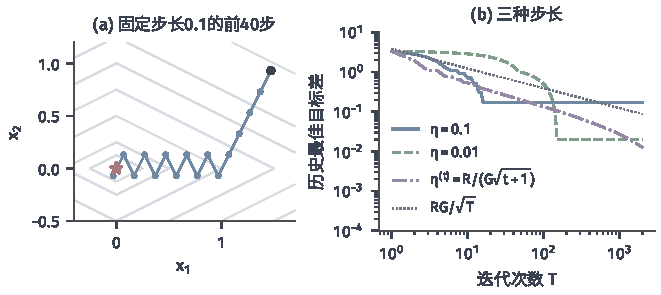
\includegraphics[width=112mm]{figures/03-optimization-evolution-and-signals/01-optimization/matplotlib/c4-subgrad-steps/figure.pdf}
  \caption{次梯度法的步长与锯齿。目标$f(\bm x)=|x_1|+2|x_2|$，最小点为原点（红星），初值$(1.47,0.93)^\top$。(a) 固定步长$\eta=0.1$的前40步：到达横轴附近后在两侧来回跳动。(b) 历史最佳目标差随迭代次数的变化（双对数坐标）：固定步长$0.1$与$0.01$分别停在约$0.17$与$0.02$的平台，递减步长$\eta^{(t)}=R/(G\sqrt{t+1})$持续下降；灰色点线为参考量$RG/\sqrt T$。}
  \label{fig:opt-ns-subgrad-steps}
\end{figure}

\paragraph{几种量不能互相替代}
次梯度法的分析中出现了几个容易混淆的量。累计步长$\sum_t\eta^{(t)}$是摊薄初始距离所需的“时间”；实际路径长度$\sum_t\eta^{(t)}\lVert\bm g^{(t)}\rVert_2$还含次梯度范数，在锯齿阶段会持续增长；目标误差是定理~\ref{thm:opt-ns-subgradient-rate}控制的对象；参数$\bm x^{(t)}$是否收敛到某个最小点，又是另一回事。上面的定理只给出返回点的目标误差，没有断言迭代序列收敛，也没有断言路径长度有限。在锯齿例中，路径长度随步数线性增长，目标误差却停在平台：二者都不能代替对方说明算法的状态。
